\documentclass[a4paper,11pt,oneside]{book}

% PACCHETTI
\usepackage{hyperref}           % hyperlinks
\usepackage{tabto}              % strumento per inserire tab nel testo
\usepackage[                    % geometria della pagina
    a4paper,
    inner=2cm,
    outer=3cm,
    top=3cm,
    bottom=3cm,
    bindingoffset=1.2cm,
    headheight=14.5pt
]{geometry}
\usepackage[utf8]{inputenc}     % 3 pacchetti per l'italiano
\usepackage[italian]{babel}
\usepackage[T1]{fontenc}
\usepackage{titlesec}           % custom chapter titles

\usepackage{fancyhdr}
\usepackage{multicol}
\usepackage[arrowdel]{physics} 
\usepackage{amsmath}
\usepackage{tikz}
\usepackage{varwidth}

\usepackage{graphicx}           % IMMAGINI
\graphicspath{ {./images/} }

\usepackage{csquotes}
\usepackage{caption}

% INFORMAZIONI SUL DOCUMENTO
\title{\Large{\textbf{Architettura degli Elaboratori}} \\ Secondo semestre}

\author{Enrico Bragastini}
\titleformat{\chapter}[display]{\normalfont\bfseries}{}{0pt}{\LARGE}
\date{}


% CONTENUTO
\begin{document}
\pagestyle{fancy}
\fancyhf{}
\rhead{}
\lhead{\nouppercase\leftmark}
\cfoot{\thepage}
\frontmatter

% Prima pagina - Titolo
\maketitle
\tableofcontents

\mainmatter
\chapter{Introduzione}
\section{Modello di Von Neumann}
L'architettura di Von Neumann è una tipologia di architettura hardware per computer digitali programmabili
a programma memorizzato la quale condivide i dati del programma e le istruzioni del programma nello stesso spazio di memoria.

~\newline
Lo schema si basa su 5 componenti fondamentali:
\begin{itemize}
    \item \textbf{CPU} (\emph{Central Processing Unit}), una grande \emph{FSMD} che si divide a sua volta in unità aritmetica
          e logica (ALU o unità di calcolo) e unità di controllo
    \item \textbf{Memoria}, il luogo dove la CPU recupera istruzioni e dati, contenuti assieme
    \item \textbf{Bus}, il canale di comunicazione tra tutte le componenti dell'architettura. Permette alla CPU di leggere e di scrivere sulla memoria e
          di acquisire o mostrare dati comunicando con le unità di I/O.
    \item \textbf{Unità di Input/Output}, ovvero i dispositivi di input e output che permettono all'utente di interfacciarsi con la macchina (e viceversa).
\end{itemize}

\subsection{CPU (Central Processing Unit)}
La CPU è l'unità o sottosistema logico e fisico che sovraintende alle funzionalità logiche di elaborazione principali del computer.

Tutte le istruzioni che la CPU è in grado di riconoscere e di eseguire fanno parte del suo \textbf{ISA} (\emph{Istruction Set Architecture}), che è in
rapporto 1:1 con i codici binari delle istruzioni stesse che vengono eseguite, ad ogni istruzione corrisponde una codifica binaria che il processore
è in grado di eseguire. Se due CPU hanno ISA differenti, non potranno eseguire lo stesso sorgente, sarà quindi necessario ricompiarlo separatamente per ogni rispettivo ISA.

In certi casi è possibile che CPU diverse abbiano architetture diverse ma condividano lo stesso ISA. È il caso di \emph{Intel}, che dal processore \emph{80396} ha mantenuto
lo stesso set di istruzioni.

\newpage
\subsection{Dal codice di alto livello al binario eseguibile}
Il processo che avviene quando si compila e si esegue del codice di alto livello, come il C++, è rappresentato nel seguente schema:

\begin{figure*}[h]
    \centering
    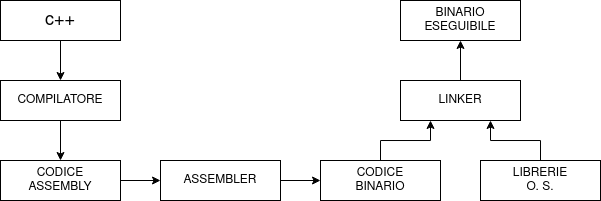
\includegraphics[scale=0.5]{da_codice_a_binario}
\end{figure*}
Il codice C++ viene compilato dal \textbf{compilatore} (GCC in questo caso), il quale produce il relativo \textbf{codice assembly}. Questo codice
deve essere \emph{assemblato} dall'\textbf{assembler} in modo da ottenere del codice binario eseguibile sulla macchina in base alle specifiche dell'\emph{ISA}.

Affinché il codice possa essere eseguito, tenendo a mente che verrà eseguito su una macchina gestita da un Sistema Operativo, è necessario includere i collegamenti alle
librerie di sistema richieste dal programmatore in fase di scrittura del codice. A questo proposito interviene il \textbf{linker}, che produrrà finalmente un \textbf{binario eseguibile}.
Il binario prodotto a questo punto è \emph{specifico per quell'ISA} e, per via delle librerie, è anche \emph{specifico per quel Sistema Operativo}.

\section{Una CPU didattica}

\begin{figure*}[h]
    \centering
    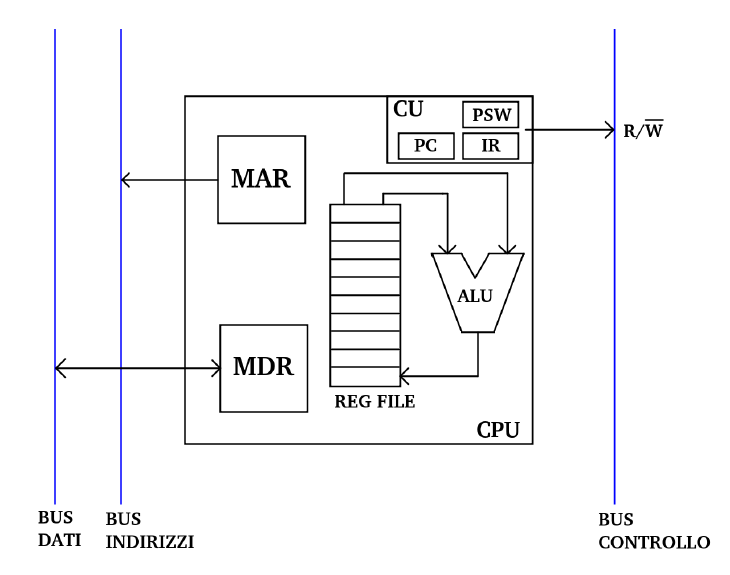
\includegraphics[scale=0.5]{cpu_didattica_schema}
\end{figure*}
\newpage
\subsubsection{Interazione con la memoria}
Per interagire con la memoria la CPU ha a disposizione i registri \emph{MAR} e \emph{MDR}, dove comunica
i dati da scrivere e dove scriverli. Per la comunicazione effettiva vengono utilizzati 3 diversi BUS.

~\newline
\textbf{Registri}:
\begin{itemize}
    \item \textbf{MAR} (\emph{Memory Address Register}): Contiene l'indirizzo di memoria con cui la CPU vuole interagire
    \item \textbf{MDR} (\emph{Memory Data Register}): Contiene il dato oggetto di scambio, ovvero ciò che viene letto da memoria o che è necessario scrivere sulla memoria
\end{itemize}

\noindent \textbf{Bus}:
\begin{itemize}
    \item \textbf{Bus Indirizzi}): Su questo Bus la CPU ci mette gli indirizzi delle celle di memoria con cui vuole operare. La CPU scrive su questo bus e non viceversa.
    \item \textbf{Bus Dati}: Bus adibito al trasferimento dei dati da e verso la memoria. Entrambe la CPU e la memoria leggono e scrivono su questo canale.
    \item \textbf{Bus di Controllo}: Bus in cui la CPU scrive i comandi che devono essere dati alla memoria. I comandi \emph{read} e \emph{write} faranno sapere alla memoria
          se la CPU ha bisogno di scrivere o di leggere.
\end{itemize}

\subsubsection{Unità di Controllo}
L'unità di controllo \textbf{CU} è una \emph{Macchina a Stati Finiti} che gestisce le fasi di ogni operazione. Si occupa di alzare/abbassare tutti i segnali interni di controllo
nel momento giusto.

All'interno della CU sono presenti 3 registri specifici:
\begin{enumerate}
    \item \textbf{PC} (\emph{Program Counter}): Registro che contiene l'indirizzo della prossima istruzione da eseguire
    \item \textbf{IR} (\emph{Istruction Register}): Registro che contiene la \emph{codifica} dell'istruzione corrente da eseguire
    \item \textbf{PSW} (\emph{Program Status Word}): Registro che contiene una serie di bit specifici, ovvero una serie di informazioni riguardo l'istruzione appena
          eseguita, utili durante l'esecuzione della successiva.
\end{enumerate}

\subsubsection{ALU (\emph{Arithmetic Logic Unit})}
È la sezione della CPU che sa svolgere tutte le operazioni logiche e aritmetiche. È come un grande Datapath controllato dalla sua FSM, ovvero l'Unità di Controllo.
La ALU, in base ai comandi della CU, prende i dati dai Registri, esegue l'operazione dovuta e ripone il risultato in un registro.

\section{Ciclo Fetch-Decode-Execute}
In termini generali, un processore esegue \underline{\emph{iterativamente}} \textbf{tre operazioni}:
\begin{enumerate}
    \item \textbf{Fetch}: È la fase di caricamento, la CPU carica dalla memoria la prossima istruzione da eseguire.
          Viene letta la cella memoria il cui indirizzo è contenuto nel \emph{Program Counter}. A questo punto l'istruzione è salvata nell'\emph{Istruction Register} e il PC viene incrementato.
    \item \textbf{Decode}: È la fase di decodifica dell'istruzione. Viene letto l'Istruction Register per capire cosa è necessario fare. Vengono eventualmente letti anche i valori necessari dalla memoria.
    \item \textbf{Execute}: È la fase di esecuzione vera e propria dell'istruzione. La ALU esegue i calcoli necessari e i registri vengono modificati.
\end{enumerate}

\section{Architettura della CPU}
\begin{figure*}[h]
    \centering
    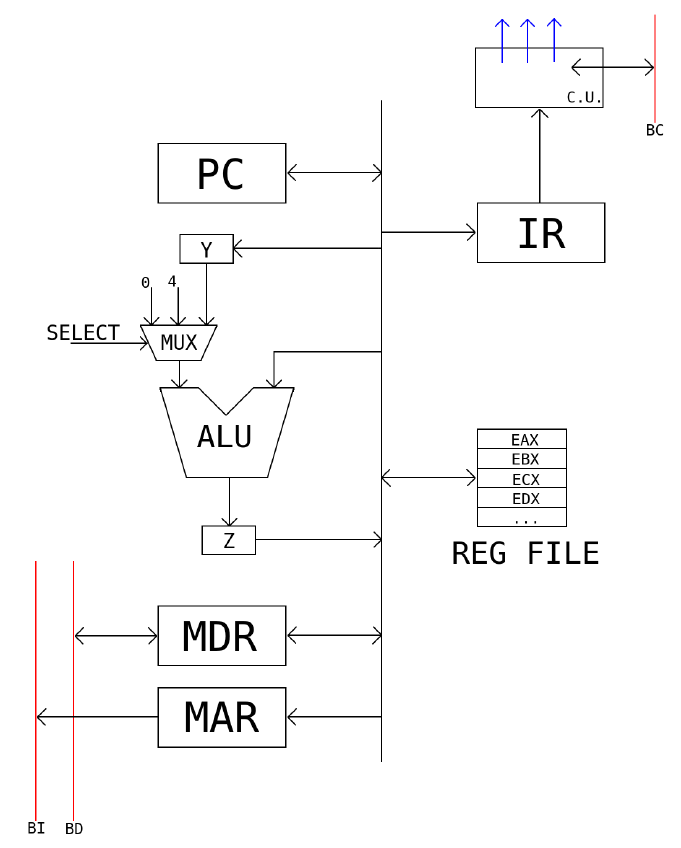
\includegraphics[scale=0.6]{modello_architettura_cpu}
\end{figure*}

\section{Assembly}
Il linguaggio Assembly è un linguaggio di programmazione molto simile al linguaggio macchina, pur essendo differente rispetto a quest'ultimo.

~\newline
È concettualmente composto di due parti:
\begin{enumerate}
    \item \textbf{ISA}, ovvero le caratteristiche del linguaggio: le \textbf{istruzioni} e i \textbf{metodi di indirizzamento}.
    \item \textbf{Sintassi}, ovvero le regole con cui va scritto il linguaggio.
\end{enumerate}
Il linguaggio Assembly da noi utilizzato sarà l'\textbf{Intel 80x86} con sintassi \textbf{AT\&T}.

\subsection{Metodi di Indirizzamento}
Il metodo di indirizzamento dice alla CPU con che modalità deve \emph{recuperare} il dato che le serve per lavorare.

\subsubsection{Indirizzamento Diretto a Registro}
In questo metodo di indirizzamento, il registro viene usato in modo \emph{esplicito}. Basterà quindi usare il nome del registro come operando Affinché
si vada ad operare con lo spazio di memoria del registro stesso

~\newline
\underline{Esempio:} \tabto{3cm} \texttt{MOVL \%EAX, \%EBX}


\subsubsection{Indirizzamento Immediato}
In questo metodo di indirizzamento, una costante viene codificata nell'istruzione stessa, utilizzando il simbolo ''\$''.
\newline \emph{Attenzione}: una costante non può essere una destinazione e quindi non può essere il secondo operando.

~\newline
\underline{Esempio:} \tabto{3cm} \texttt{MOVL \$8, \%ECX}


\subsubsection{Indirizzamento assoluto}
In questo metodo di indirizzamento viene fatto l'uso di \textbf{etichette}, la quale rappresenta un indirizzo della memoria con il quale si vuole operare.
\newline Sarà l'\emph{Assembler} ad occuparsi di sostituire il nome dell'etichetta con l'effettivo indirizzo di memoria.

~\newline
\underline{Esempio:} \tabto{3cm} \texttt{MOVL DATA, \%EBX}


\subsubsection{Indirizamento Indiretto a Registro}
In questo metodo di indirizzamento, si fa utilizzo di un \emph{indirizzo di memoria} contenuto all'interno di un registro. Per accedervi si specifica
il nome del registro all'interno di parentesi tonde.

~\newline
\underline{Esempio:} \tabto{3cm} \texttt{MOVL (\%EAX), \%EBX}

\subsubsection{Indirizzamento Indiretto a Registro con Spiazzamento}
In questo metodo di indirizzamento, si utilizza sempre un \emph{indirizzo di memoria}, contenuto all'interno di un registro, a cui viene sommata una costante, chiamata \textbf{spiazzamento}.

~\newline
\underline{Esempio:} \tabto{3cm} \texttt{MOVL \$4(\%EAX), \%EBX}


\subsection{Istruzioni}
Le istruzioni possono avere una \textbf{codifica fissa} oppure una \textbf{codifica variabile}.
A scopo didattico lavoreremo con istruzioni a codifica fissa.

\noindent La struttura di un'istruzione è del tipo \emph{OPCODE OPER1, OPER2} dove:
\begin{itemize}
    \item \textbf{OPCODE} è il nome dell'istruzione stessa. Un certo numero di bit dell'istruzione definiscono qual è l'operazione Assembly da eseguire.
    La definizione dell'insieme degli \emph{opcode} fa parte dell'\emph{ISA}.    
    \item \textbf{OPER1} è il primo operando dell'istruzione. In certe operazioni è anche l'unico operando.
    \item \textbf{OPER2} è il secondo operando dell'istruione. Quando presente, rappresenta anche la \emph{destinazione} dell'operazione, ovvero dove
          verrà salvato il risultato.
\end{itemize}

\noindent Alcuni esempi di istruzioni:
\begin{itemize}
    \item Operazioni con la memoria
    \begin{itemize}
        \item \texttt{MOVL}: Permette lo spostamento di dati dalla memoria ai registri (e viceversa) e tra i registri stessi.
        \item \texttt{PUSHL / POPL}: Permettono la gestione dello \underline{stack}
    \end{itemize}
    \item Operazioni Aritmetiche
    \begin{itemize}
        \item \texttt{ADDL}: operazione di somma
        \item \texttt{SUBL}: operazione di sottrazione
    \end{itemize}
    \item Gestione del flusso operativo
    \begin{itemize}
        \item \texttt{CMPL}: compara due dati. Dopo la comparazione viene modificato il bit apposito nel registro PSW
        \item \texttt{JMP}: Operazione di \emph{salto} a un'istruzione diversa dalla successiva. Ne esistono varie derivate
        \begin{itemize}
            \item \texttt{JG}: salta se maggiore
            \item \texttt{JL}: salta se minore
            \item \texttt{JE}: salta se uguale
            \item \texttt{JGE}: salta se maggiore o uguale
            \item \texttt{JLE}: salta se minore o uguale
            \item \texttt{JZ}: salta se uguale a zero
            \item \texttt{JNZ}: salta se diverso da zero
            \item \texttt{JMP}: salto incondizionato
        \end{itemize}
        \item \texttt{CALL}: chiamata a sottoprogramma, definito da una \emph{etichetta}. Dopo l'esecuzione del sottoprogramma si prosegue con l'istruzione successiva (mediante la chiamata dell'istruzione \texttt{ret}).
    \end{itemize}
    \item \texttt{NOP}: operazione nulla che non effettua niente. È utile in certe situazioni particolari
\end{itemize}


\subsection{Microistruzioni}
Ogni istruzione Assembly viene eseguita in più passi minori. Innanzitutto perché ogni istruzione viene eseguita dalla CPU in tre fasi (\emph{fetch}, \emph{decode}
ed \emph{execute}) e ognuna di queste fasi corrisponde a un insieme di \textbf{microistruzioni} eseguite internamente dalla CPU.

~\newline
\underline{Esempio - Indirizzamento diretto a registro:} \tabto{9cm} \texttt{ADDL \%EAX, \%EBX}
\begin{enumerate}
    \item Fetch: \texttt{PCout, MARin, READ, SELECT4, ADD, Zin} \newline
          Il valore in PC viene "lasciato uscire" sul bus e "fatto entrare" in MAR. Viene dato il segnale di READ alla memoria per leggere la prossima istruzione. SELECT4, ADD e Zin permetteranno PC (gli viene aggiunto il valore 4 mediante la ALU)

    \item Fetch: \texttt{WMFC, Zout, PCin} \newline
          Viene \emph{messo in pausa} il clock della CPU in attesa che la memoria recuperi il dato e lo scriva sul bus dati. \newline Inoltre il valore della somma precedente viene fatto uscire dalla ALU e salvato in PC (PC è stato quindi incrementato).

    \item Fetch: \texttt{MDRout, IRin} \newline
          Il valore dalla memoria è stato scritto sul bus e quindi in MDR. Il dato viene fatto "uscire" da MDR e viene fatto "entrare" in IR. A questo punto l'istruzione da eseguire è stata \emph{caricata} ed è pronta per essere eseguita.

    \item Execute: \texttt{EAXout, Yin} \newline
          Il valore presente in EAX viene scritto nel registro Y in ingresso alla ALU.

    \item Execute: \texttt{EBXout, SELECTy, ADD, Zin} \newline
          Il valore in EBX viene fatto "uscire" sul bus e quindi è già leggibile dalla ALU. A questo punto il mux lascia passare il valore di Y nell'altro ingresso della ALU e il segnale ADD fa eseguire la somma tra i due valori. Il risultato viene fatto entrare in Z.

    \item Execute: \texttt{Zout, EBXin, END} \newline
          Il valore ottenuto dalla somma che si trova in Z viene quindi salvato nel secondo operando, ovvero EBX. Il segnale di END comunica il compimento dell'istruzione.
\end{enumerate}
Essendo i valori da sommare già presenti nei registri, ovvero entrambi con \emph{indirizzamento diretto a registro}, la fase di decode non è necessaria: i valori sono già pronti per essere utilizzati dalla ALU.

~\newline
\underline{Esempio - Indirizzamento indiretto a registro:} \tabto{9cm} \texttt{ADDL (\%EAX), \%EBX}
\begin{enumerate}
    \item Fetch: \texttt{PCout, MARin, READ, SELECT4, ADD, Zin}
    \item Fetch: \texttt{WMFC, Zout, PCin}
    \item Fetch: \texttt{MDRout, IRin}
    \item Decode: \texttt{EAXout, MARin, READ}
    \item Decode / Execute: \texttt{WMFC, EBXout, Yin}
    \item Decode / Execute: \texttt{MDRout, SELECTy, ADD, Zin}
    \item Execute: \texttt{Xout, EBXin, END}
\end{enumerate}

\section{Memoria}
La sezione di memoria che il sistema operativo fornisce a un programma per l'esecuzione, la quale parte
dall'indirizzo $0$ all'indirizzo $max$, è concettualmente suddivisa in quattro parti:
\begin{enumerate}
    \item \textbf{Sezione del codice}: contiene le istruzioni del codice da eseguire
    \item \textbf{Dati statici}: contiene tutte le \emph{variabili statiche} presenti all'interno del codice. 
    \item \textbf{Heap}: è una \emph{sezione \textbf{dinamica}}, ovvero che varia durante l'esecuzione.
    Ogni volta che il programma necessita di allocare uno spazio di memoria non dimensionabile a priori, richiede al \emph{Sistema Operativo} lo spazio di cui
    ha bisogno. Quando il S.O. fornisce lo spazio richiesto, che potrebbe anche essere l'\textbf{intera memoria}, questo farà parte della sezione \emph{Heap}. È il caso di quando si utilizzano le funzioni \texttt{malloc()} e \texttt{mfree()} in C.
    \item \textbf{Stack (pila)}: è una \emph{sezione \textbf{statica}}, ovvero di dimensioni fisse, per l'allocazione di variabili dalle dimensioni statiche e
    quindi conosciute al momento della programmazione. La dimensione dello \emph{stack} ha un range che va da qualche \emph{KB} a non oltre qualche \emph{MB}, pertanto non 
    è necessario stare attenti a non saturare questa sezione di memoria.
\end{enumerate}

\subsection{Il funzionamento dello Stack}
Le \emph{word} vengono inserite all'interno dello stack a partire dal basso verso l'alto, come una \emph{pila} di piatti.
Quando si richiede di leggere dallo stack, le \emph{word} vengono recuperate dall'alto verso il basso.

Il registro \textbf{ESP} \emph{(Stack Pointer)} contiene in ogni momento il puntatore all'ultima \emph{word} inserita nello stack.

~\newline
Le istruzioni a disposizione per l'interazione con lo stack sono \texttt{PUSHL} e \texttt{POPL}:
\begin{itemize}
    \item \texttt{PUSHL <VALUE>}: viene inserito il valore all'interno dello stack e viene \emph{decrementato il registro ESP}. \newline
    Per esempio, l'istruzione \texttt{PUSHL \%EAX} corrisponde a:
    \begin{itemize}
        \item \texttt{SUBL \$4, \%ESP}
        \item \texttt{MOVL \%EAX, (\%ESP)}
    \end{itemize}
    \item \texttt{POPL <VALUE>}: viene recuperato ciò che c'è in cima allo stack e viene \emph{incrementato il registro ESP}. \newline
    Per esempio, l'istruzione \texttt{POPL \%EBX} corrisponde a:
    \begin{itemize}
        \item \texttt{MOVL (\%ESP), \%EBX}
        \item \texttt{ADDL \$4, \%ESP}
    \end{itemize}
\end{itemize}
È errato utilizzare le espressioni equivalenti di \texttt{PUSHL} e \texttt{POPL}. Questo perché per ogni istruzione abbiamo la \emph{certezza} che la CPU
porterà a termine l'istruzione senza fare altro. Tra una istruzione e un'altra noi non possiamo avere la certezza di ciò, per cui utilizzando le due istruzioni equivalenti,
tra una e l'altra la CPU potrebbe fare delle cose a noi sconosciute, portando a effetti indesiderati.





\end{document}
